\chapter{Sensoren und frequenzselektive Messverfahren}

\section{Einleitung}

\begin{table}[!h]
	\centering
	\begin{tabular}{|c|c|}
		\hline 
		Teilnehmer 		& Oskar Fürnhammer, Katharina Kralicek, Patrick Mayr \\
		\hline 
		Datum 		& 06.12.2018 \\ 
		\hline 
		Messplatzbez. 	& CA0410-1 \\
		\hline
	\end{tabular} 
	%\caption{Grundlegende Information der 6. Laborübung}
\end{table}

\begin{table}[!h]
	\centering
	\begin{tabular}{ c | c }

Gerät				& Bezeichnung		\\
\hline

Spannungsquelle		& Rigol DP832			\\
Oszilloskop			& Agilent DSO-X 2002A		\\
Breakout-Box		& Agilent U2542A 			\\

	\end{tabular}

	\caption{Verwendete Geräte}
\end{table}

\newpage

\section{Kennlinie des Näherungssensors}

Hierbei sollte für zwei Reflektoren unterschiedlicher Oberflächenbeschaffenheiten die Kennlinie des Näherungssensors aufgenommen werden. Der Näherungssensor wurde symmetrisch mit 12V versorgt, die LED mit 1,5V aus dem Funktionsgenerator des Oszilloskops, und der Ausgang des Sensors wurde mit dem Oszilloskop sowie der Breakout-Box verbunden.
\begin{figure}[h]
	\centering
	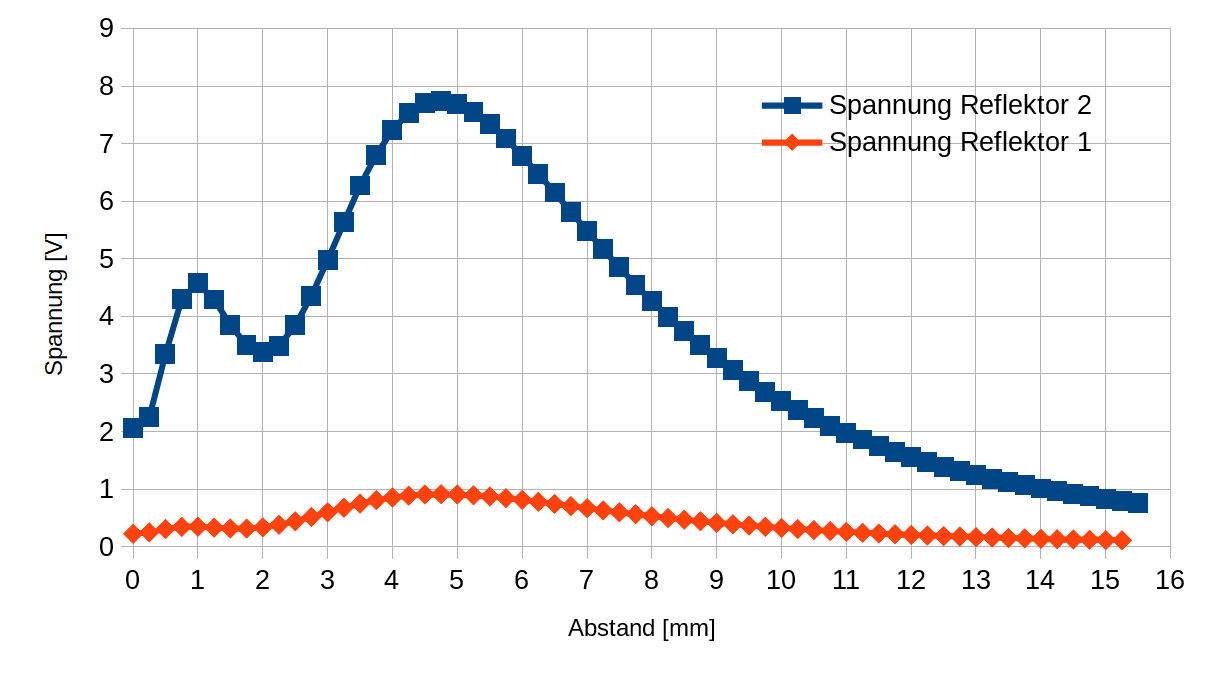
\includegraphics[width=0.8\textwidth]{./img/ch6/Kennlinie_Reflektor_1_und_2}
	\caption{Kennlinie Reflektor 1 und 2}
	\label{fg:kenn_refl}
\end{figure}
~\\
Wie in Abb. \ref{fg:kenn_refl} ersichtlich haben die gemessenen Kennlinien bei beiden Reflektoren die gleiche Form, jedoch sind die Spannungswerte bei Reflektor 2 deutlich höher. Das lässt auf eine glattere, und damit besser reflektierende Oberfläche schließen.
\begin{figure}[h]
	\centering
	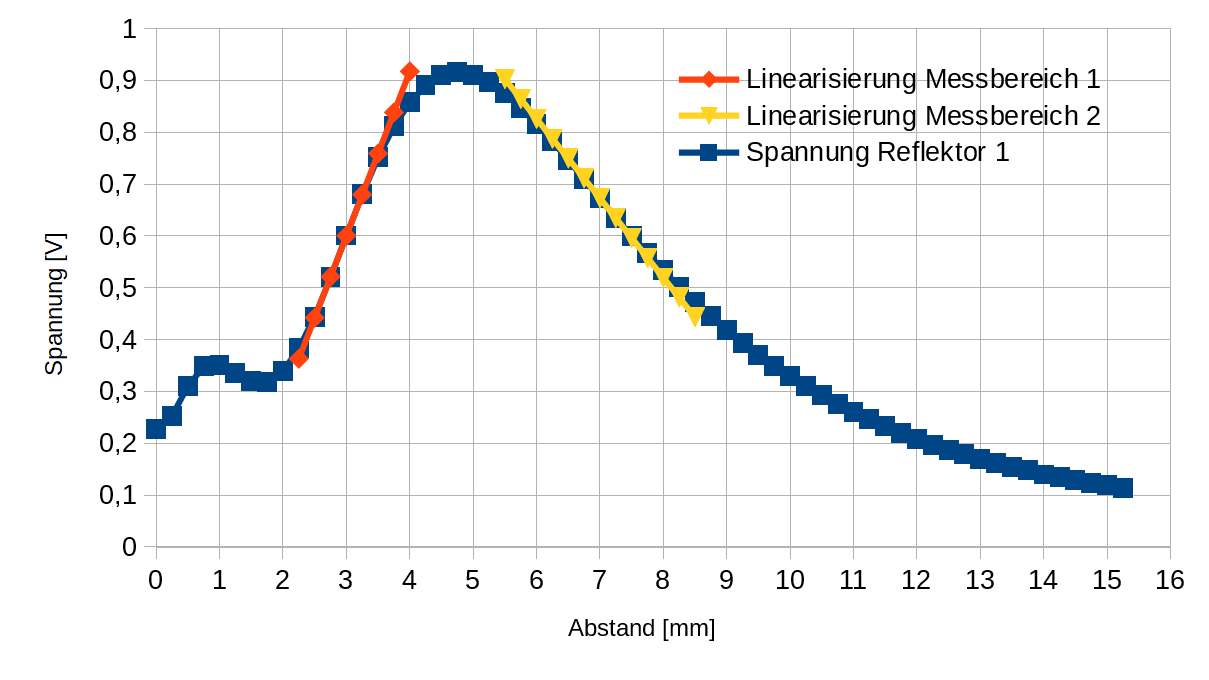
\includegraphics[width=0.8\textwidth]{./img/ch6/Linearisierung_Reflektor_1}
	\caption{Linearisierung Reflektor 1}
	\label{fg:kenn_linear1}
\end{figure}
~\\\begin{figure}[h]
	\centering
	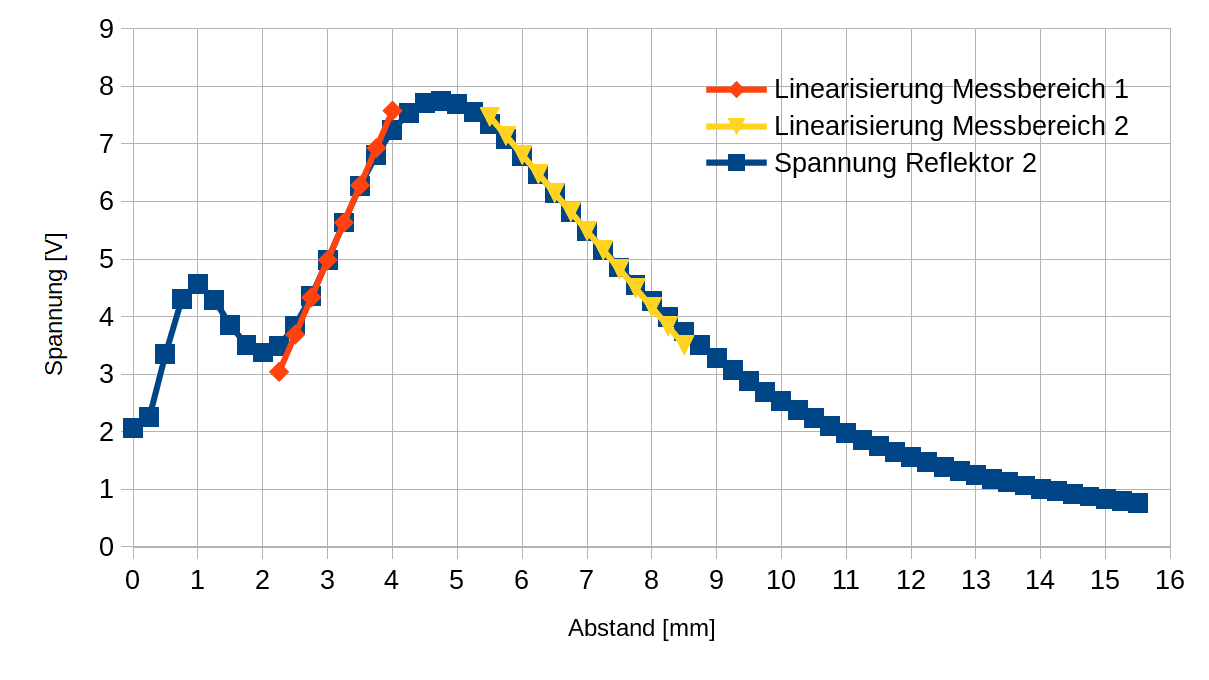
\includegraphics[width=0.8\textwidth]{./img/ch6/Linearisierung_Reflektor_2}
	\caption{Linearisierung Reflektor 2}
	\label{fg:kenn_linear2}
\end{figure}
~\\
Für beide Reflektoren wurden in Abb. \ref{fg:kenn_linear1} und \ref{fg:kenn_linear2} die Bereiche gekennzeichnet, in denen die Kennlinie annähernd linear verläuft. Ihre Gleichungen lauten für Reflektor 2 im Messbereich 1 $U = 2,592(V/mm) \cdot x - 2,791V$ und im Messbereich 2 $U = -1,324(V/mm) \cdot x + 14,755V$, und für Reflektor 1 im Messbereich 1 $U = 316,8(mV/mm) \cdot x - 349,5mV$ und im Messbereich 2 $U = -153,2(mV/mm) \cdot x + 1,7454V$. Aus diesen Gleichungen kann man die Sensitivität E der Messbereiche ablesen, diese entspricht der jeweiligen Steigung. Es ergibt sich, das die Sensitivität im Messbereich 1 des Reflektors 2 mit 2,592(V/mm) am höchsten ist.
\begin{figure}[h]
	\centering
	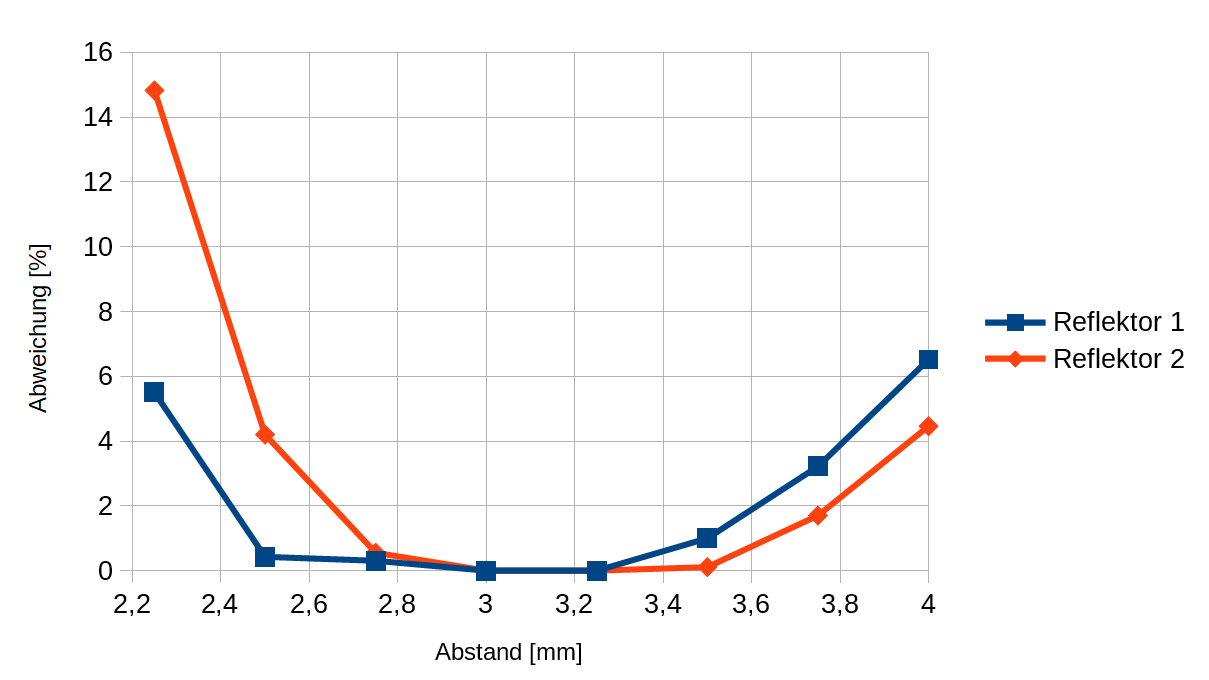
\includegraphics[width=0.8\textwidth]{./img/ch6/Prozentuelle_Abweichung_Kennlinie_Linearisierung_Messbereich_1}
	\caption{Prozentuelle Abweichung Kennlinie Linearisierung Messbereich 1}
	\label{fg:kenn_mb1}
\end{figure}
~\\
\begin{figure}[h]
	\centering
	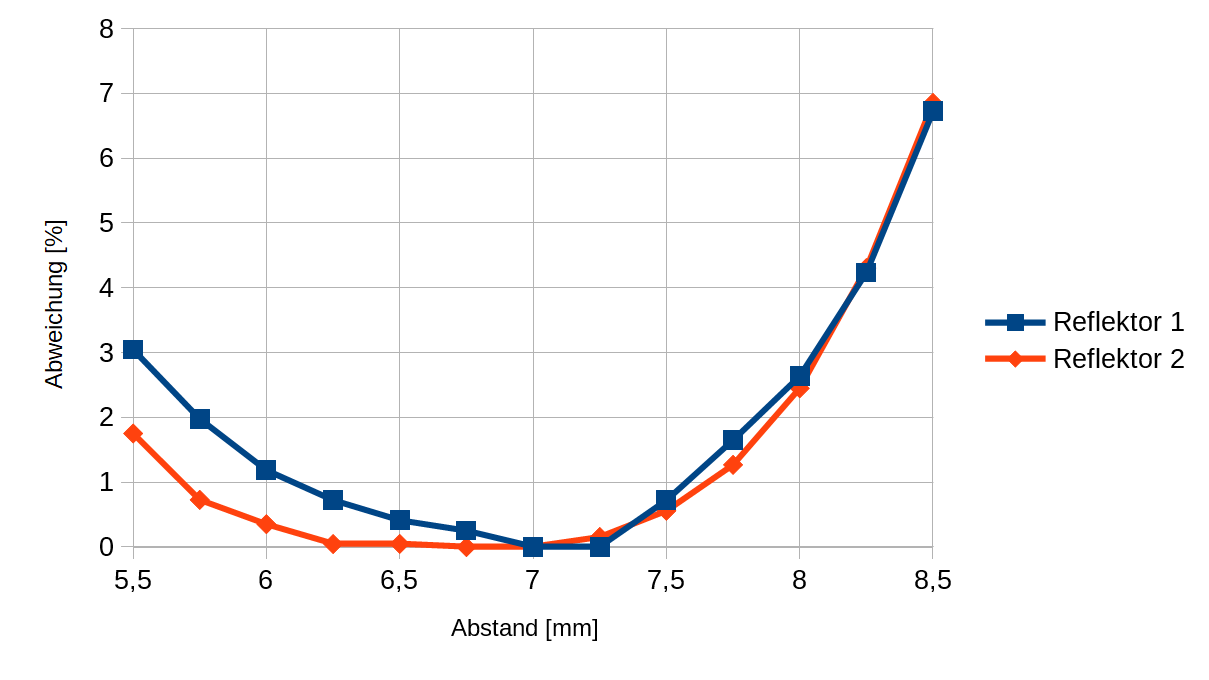
\includegraphics[width=0.8\textwidth]{./img/ch6/Prozentuelle_Abweichung_Kennlinie_Linearisierung_Messbereich_2}
	\caption{Prozentuelle Abweichung Kennlinie Linearisierung Messbereich 2}
	\label{fg:kenn_mb2}
\end{figure}
~\\
Die Abweichungen der Messpunkte von der Gerade sind in Abb. \ref{fg:kenn_mb1} und Abb. \ref{fg:kenn_mb2} dargestellt. Hierbei kann man sehen, dass die Abweichung für den Reflektor 1 im Messbereich 1 bei einem Abstand von 4mm und im Messbereich 2 bei einem Abstand von 8,5mm zum Sensor maximal wird, und für den Reflektor 2 im Messbereich 1 bei einem Abstand von 2,25mm und im Messbereich 2 bei einem Abstand von 8,5mm zum Sensor maximal wird. Da die Kennlinie des Sensors durch die Messpunkte interpoliert werden kann, ist somit keine weitere Linearisierung notwendig. Dadurch kann man den Sensor in sämtlichen Messbereichen betreiben, solange man darauf achtet, dass die Kennlinie darin eindeutig bleibt, sich also Messwerte für verschiedene Abstände nicht wiederholen. Dadurch ergibt sich prinzipiell der Messbereich rechts vom Maximum als am besten geeignet für Messungen.

\section{Rauschen und Auflösung}

Die Messung für Rauschen und Auflösung fand bei eingeschalteter Deckenbeleuchtung und bewölktem, bereits leicht dämmernden Himmel statt, bei aufgedrehtem Monitor des Computers. Das Schaltbild in Simulink, zu sehen in Abb. \ref{fg:schalt_rauschen} wurde um die Messung der Standardabweichung und des Spitze-Spitze-Wert erweitert, bevor die Messung begonnen wurde. Der Abstand des Reflektors zum Sensor wurde  5mm gewählt. In Tabelle \ref{tb:messerg} finden sich alle Messergebnisse.
\begin{figure}[h]
	\centering
	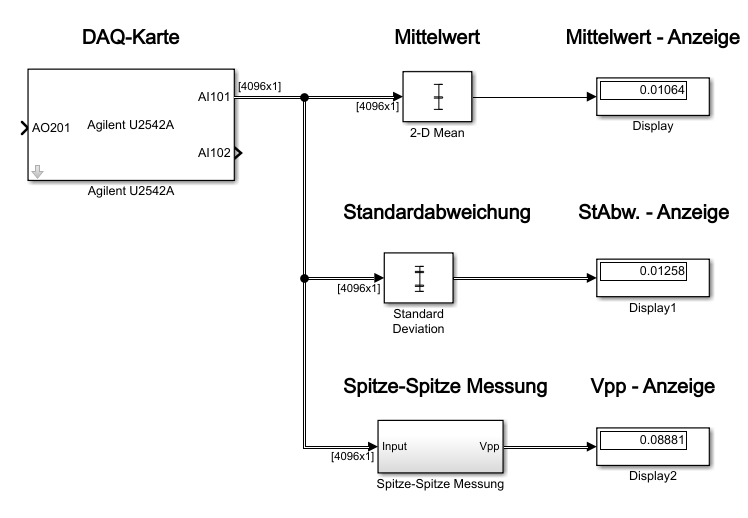
\includegraphics[width=0.8\textwidth]{./img/ch6/6_3_3}
	\caption{Schaltbild}
	\label{fg:schalt_rauschen}
\end{figure}
~\\
\begin{table}[!h]
	\centering
	\begin{tabular}{|c|c|c|}
	\hline 
	Messgrößen [V]			& $U_e$ = 1,5		& $U_e$ = 0,5 	\\ 
	\hline 
	Mittelwert [V]			& 7,645			& 2,097	\\ 
	\hline 
	Standardabweichung [1]		& 0,01368			& 0,01351	\\ 
	\hline 
	Spitze-Spitze-Spannung [V]	& 0,1117			& 0,9308	\\ 
	\hline 
	\end{tabular}
	%\caption{Einstellungen des Frequenzsgenerators}
	\label{tb:messerg}
\end{table}
~\\
Man erkennt, dass die angelegte Gleichspannung die Messung den Mittelwert und die Spitze-Spitze-Spannung maßgeblich beeinflusst.
~\\
Die aus der Gleichung $U_{pp} = 6 \cdot \sigma$ errechnete Spannung $U_{pp} = 0,082V$ für $U_e = 1,5V$ und $U_{pp} = 0,081V$ für $U_e = 0,5V$ entspricht nahezu der gemessenen $U_{pp}$ Spannung, womit die Verteilung ähnlich einer Gaußschen Verteilung ist.
~\\
Allgemein als Quellen von Rauschen sind das Tageslicht, die Beleuchtung im Raum, die Schaltung, die Raumtemperatur, sowie jede Umwandlung eines analogen Signals in ein digitales zu betrachten. Das Rauschen kann folglich beispielsweise durch Abschirmung des Sensors gegenüber unerwünschter Lichtquellen oder elektromagnetischer Felder verringert werden, genauso kann man den Raum um den Sensor abkühlen und die Datenverarbeitung anders gestalten.
~\\
Die Positionsauflösung errechnet sich mit der Formel $\Delta x = \dfrac{\sigma}{E}$ für eine Eingangsspannung von $U_e = 1,5V$ im Messbereich 1 für Reflektor 2 zu $\Delta x = 5,278\mu m$.

\section{Spektrum der Fremdlichtintensität}

\begin{figure}[h]
	\centering
	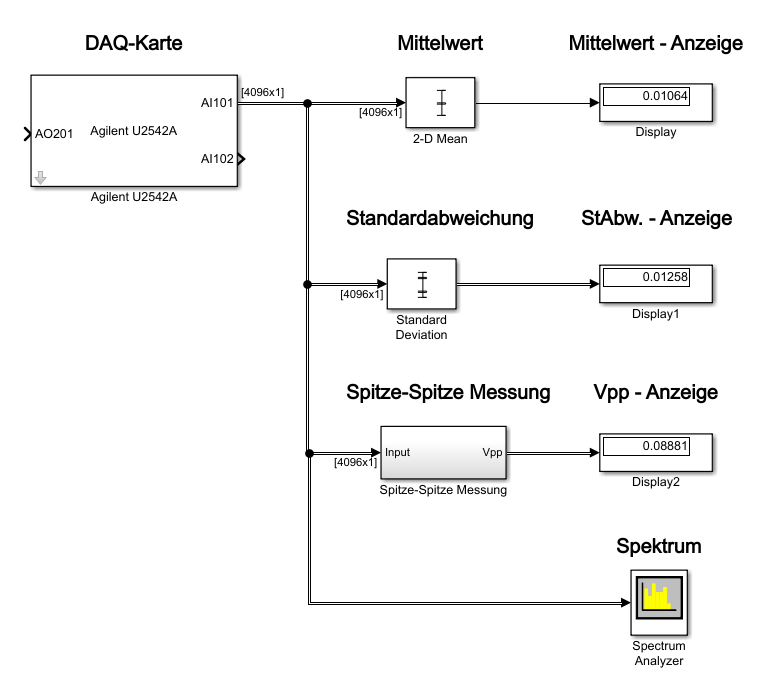
\includegraphics[width=0.8\textwidth]{./img/ch6/6_3_4}
	\caption{Schaltbild zur Berechnung des Spektrums der Fremdlichtintensität}
	\label{fg:schalt_spek}
\end{figure}
~\\
Bei dieser Messung sollte anhand einer Glühfadenlampe, sowie der Deckenbeleuchtung, konkret Leuchtstoffröhren, das Spektrum von Fremdlichtintensitäten ermittelt werden. Dazu wurde die Sender-LED mit 0V gespeist, um rein den Einfluss äußerer Lichtquellen im Spektrum zu sehen. Zusätzlich wurde das Schaltbild in Simulink um einen Spectral Analyzer erweitert.
~\\
Bei eingeschalteter Deckenbeleuchtung und eingeschalteter Glühfaserlampe erkennt man sehr gut die Auswirkung der Glühfaserlampe im Frequenzspektrum anhand der zwei Peaks bei -100Hz und 100Hz, sowie dem Peak bei Null Hz. Diese ergeben sich aus der Netzfrequenz, da die Intensität des Lichts durch die Leistung bestimmt wird, die sich wie folgt errechnet:
\begin{equation}
	 P = \dfrac{U^2}{R} = \dfrac{sin(wt)^2}{R} = \dfrac{1}{2} \cdot \dfrac{1 - cos(2wt)}{R}.
	%\label{eq:sens}
\end{equation}
~\\
Bei ausgeschalteter Glühfaserlampe und eingeschalteter Deckenbeleuchtung sah man den Peak bei 0Hz und ganz schwach Erhöhungen der Amplitude bei $\pm 100Hz$, sowie eine seltsame Verformung des Frequenzspektrums.
~\\
Zusätzlich ist noch aufgefallen, dass die Glühfaserlampe des Nachbartisches, die zwei bis drei Meter entfernt von dem Sensor stand, auf das Frequenzspektrum einen nahezu gleich ausgeprägten Einfluss hatte, wie die direkt darüber platzierte Glühfaserlampe.
~\\
!!! oskar: Abb. (6 3 4 mitTischleuchte mitDeckenleuchte (bitte irgendwo weiter hinten im Kapitel einbinden)!!!!
~\\
\section{Phasenselektiver Synchrongleichrichter (PSSG)}

\begin{figure}[h]
	\centering
	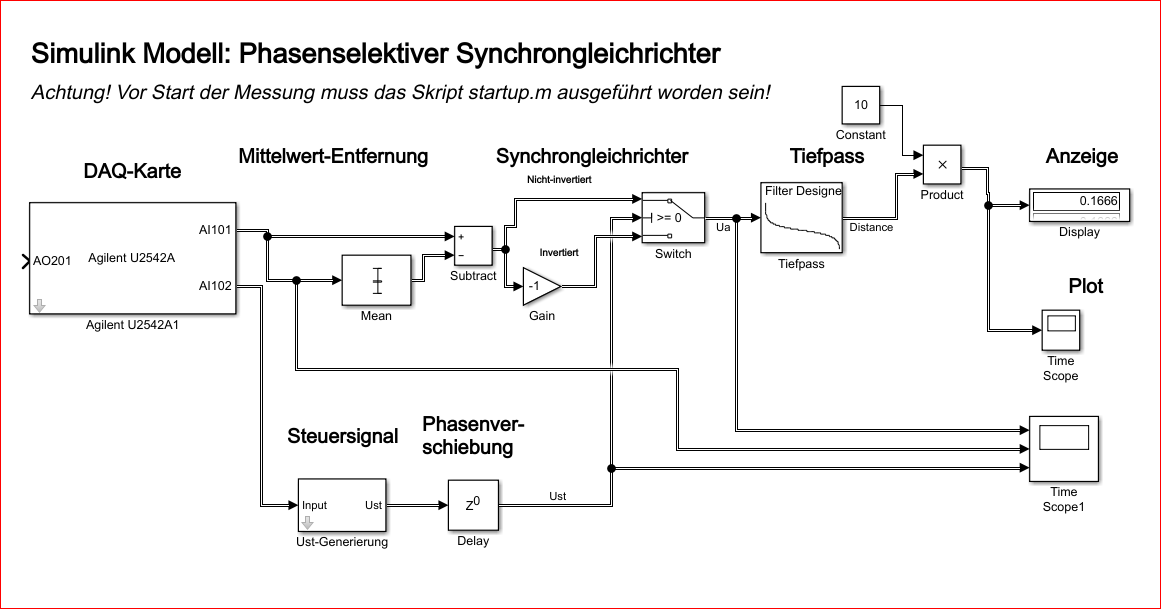
\includegraphics[width=0.8\textwidth]{./img/ch6/6_3_5}
	\caption{Schaltbild PSSG}
	\label{fg:schalt_pssg}
\end{figure}
~\\
Es sollte die Funktionsweise eines PSSG ermittelt werden. Das Schaltbild in Simulink wurde erneut entsprechend verändert, zusätzlich wurde am Funktionsgenerator ein Sinussignal mit Amplitude 0,4V und Offset 1,3V eingestellt. Als Verstärkung wurde 10 gewählt.
~\\
Der Synchrongleichrichter braucht ein Steuersignal, das festlegt, wann das Messsignal invertiert wird. Eine korrekte Messung der Amplitude des Eingangssignals ist nur möglich, wenn zwischen dem Steuersignal und dem Messsignal eine Phasenverschiebung von $\varphi= 0^\circ $ herrscht. Ist dies nicht so, dann gelingt die Mittelwertbildung nicht korrekt und das Messergebnis ist falsch.
~\\
Die Phasenverschiebung wurde durch ein Verzögerungsglied eingestellt. Die dafür erforderlichen Schritte errechnen sich durch $\Delta t = \dfrac{\varphi}{2} \cdot \pi \cdot f$ zu Schritte = $\dfrac{\Delta t}{Ta}$ !!! korrekt?!!!!. Für $45^\circ$  ergibt das 33,4, also 33 Schritte, für $90^\circ$  66,6, folglich 67 Schritte.
~\\
!!! oskar: Abb. (6 3 5 67s 1 (bitte nach den Phasen einbauen) = Phase 90Grad verschoben)!!!!
~\\
Nun sollte noch der Einfluss von Störungen auf die Messung betrachtet werden. Immer, wenn die Störfrequenz gleich ist der Messfrequenz, wird das Messergebnis beeinflusst. Dabei müssen auch die harmonischen Oberschwingungen des Rechtecksignals berücksichtigt werden, die der Synchrongleichrichter zum Invertieren des Signales benötigt. Andere Störeinflüsse, die weder mit der Frequenz des Messsignals, noch mit einer Harmonischen des Rechtecks zusammenfallen, werden sehr gut gefiltert und beeinflussen damit die Messung nicht. Wichtig ist noch, dass bei der Messung der Störung nicht genau mit der Frequenz des Messsignals gemessen wird, sondern mit einer um circa 0,1 bis 0,5 Hz versetzten Frequenz, da sonst die Störung als Gleichanteil auftritt und somit schwieriger als solche erkennbar ist.
~\\
Die hierbei betrachtete Störquelle ist wieder die Glühfadenlampe, die eine Störfrequenz von $f_S = 100Hz$ hat. Erwartet wurden dadurch Störungen bei den Frequenzen 20Hz, 33,333Hz und 100Hz. Die 20Hz Störung entspricht dabei der 5. Harmonischen Oberschwingung und die 33,333Hz Störung der 7. Harmonischen Oberschwingung des Rechtecksignals.
~\\
Die Messung ergab, entsprechend der Erwartung, eine Störung bei 20,1Hz, 33Hz und bei 100,1Hz, wobei man bei 100,1Hz die Störung am deutlichsten sehen kann. Weiters wurden die Frequenzen 50,5Hz, 75,1Hz, 125,1Hz, 150,2Hz, 175,5Hz und 200,1Hz gemessen, sie wiesen jedoch alle keine Störungen auf.
~\\
!!! oskar: Abb. (6 3 5 100hz (eher am Ende einbinden, wo‘s passt) = Störung bei 100Hz)!!!!


\section{Phasenunabhängiger Synchrondemodulator (PUSD)}

\begin{figure}[h]
	\centering
	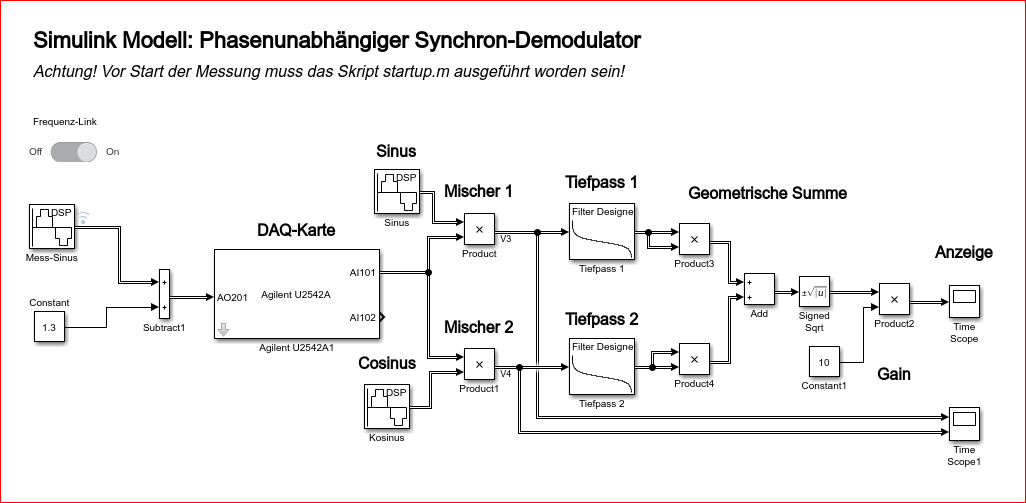
\includegraphics[width=0.8\textwidth]{./img/ch6/6_3_6}
	\caption{Schaltbild PUSD}
	\label{fg:schalt_pusd}
\end{figure}
~\\
Für den PUSD wird nun erneut das Schaltbild in Simulink verändert, ersichtlich in Abb.\ref{fg:schalt_pusd}. Das Messsignal wird nun über die DAQ Karte in die Messschaltung eingespeist, und es wird über den Block Mess-Sinus im Schaltbild am Computer generiert, mit einer Amplitude von 0,2V und einem Offset von 1,3V. Zusätzlich wird noch zur Filterung ein Butterworth-Tiefpassfilter 10. Ordnung mit Grenzfrequenz $f_g = 5Hz$ implementiert.
~\\
Dieser Filter trägt dazu bei, dass Störungen ausschließlich an der Messfrequenz, beziehungsweise bis maximal 5Hz Abweichung um die Messfrequenz zu erwarten sind, denn alle anderen Frequenzen werden mit dem nahezu idealen Butterworth-Tiefpassfilter weggefiltert. Dies bestätigte sich bei der Messung auch, wo die gleichen Frequenzen betrachtet wurden, wie auch schon im Punkt zuvor für die PSSG, und die einzige Frequenz, an der eine Störung autrat, war 101Hz.
~\\
Anhand dieser Messung kann man sehr schön den Vorteil eines PUSD gegenüber eines PSSG erkennen. Neben der schon im Namen steckenden Eigenschaft, dass der PUSD keine Information über die Phasenlage der Signale benötigt, sind Störungen tatsächlich nur an ihrer eigenen Frequenz zu erwarten, und es müssen keine möglichen Oberschwingungen eines Rechtecksignals betrachtet werden.















